\scanpage{24}
% letterhead
\begin{center}
I N S T I T U T\\
DES HAUTES ÉTUDES SCIENTIFIQUES\\
\rule{1cm}{0.4pt}
\end{center}

\handwritten{SGA 4 $\overline{\text{\uline{VII}}}$\quad p. 20}

% The spatial setting preserves the nested reference calls and their distinction
% from the comma after algébrique and the period after the first cohérent.
\figure{\begin{tikzpicture}[x=.013cm,y=-.013cm,
  every node/.style={anchor=base west,inner sep=0pt,font=\small}]
\node at (130,372) {\handwritten{\uline{Ajouter} 5.6.}};
\node at (293,350) {\handwritten{\textcircled{\scriptsize a}}};
\node at (324,369) {\handwritten{$\tilde{X}_{\mathrm{et}}$ est}};
\node at (454,363) {\handwritten{localement cohérent.}};
\node at (751,357) {\handwritten{Il est cohérent}};
\node at (985,354) {\handwritten{\deleted{\illegible{1}}}};
\node at (476,316) {\handwritten{\inserted{algébrique, d. torsion}}};
\node at (585,275) {\handwritten{\inserted{(ref)}}};
\node at (729,322) {\handwritten{\inserted{(ref)}}};
\node at (977,329) {\handwritten{\inserted{(ref)}}};
\draw[line width=.4pt] (439,370) .. controls (438,345) and (438,337) .. (453,335)
  .. controls (580,326) and (735,312) .. (824,298)
  .. controls (832,294) and (827,285) .. (822,283);
\draw[line width=.4pt] (598,330) .. controls (598,303) and (610,289) .. (631,284);
\draw[line width=.4pt] (716,374) .. controls (720,351) and (727,340) .. (741,336)
  .. controls (771,330) and (797,324) .. (810,318)
  .. controls (814,315) and (814,307) .. (811,304);
\node at (181,444) {\handwritten{(resp. quasi-séparé)}};
\node at (433,400) {\handwritten{\inserted{(ref)}}};
\draw[line width=.4pt] (452,448) .. controls (449,427) and (487,412) .. (507,386);
\node at (505,426) {\handwritten{\deleted{\illegible{1}}}};
\node at (638,423) {\handwritten{sss le schéma $X$ est}};
\node at (181,503) {\handwritten{\deleted{\unsure{quasi-cpt}}}};
\node at (337,496) {\handwritten{cohérent i.e.}};
\node at (558,484) {\handwritten{qu. cpt qu. sép}};
\node at (860,471) {\handwritten{(resp. quasi-}};
\node at (181,559) {\handwritten{séparé).}};
\node at (344,546) {\handwritten{\deleted{\illegible{1}}}};
\end{tikzpicture}}

\handwritten{\textcircled{b} Soit $(X_i)_{i\in I}$ système projectif filtrant à morphismes de transition affines, $X=\varprojlim_i X_i$ (EGA $\overline{\text{\uline{IV}}}$ 8),}

\handwritten{Âlors}
\[
\handwritten{\tilde{X}_{\mathrm{et}}\simeq\underset{\longleftarrow}{\mathrm{limtop}}\,\tilde{X}_i.}
\]

% The corollary is beside the display and above the line beginning En déduire.
% Its two added expressions have drawn enclosures; the left one has a looped
% call stroke. The small separate curve under the first et is reproduced
% without assigning a mathematical function to it.
\margin{\hspace*{-1.1cm}\begin{tikzpicture}[x=.007cm,y=-.011cm,
  every node/.style={anchor=base west,inner sep=0pt,font=\tiny}]
\node at (765,710) {\handwritten{\uline{Cor.} 5.6.1.}};
\node at (932,699) {\handwritten{$X'\in\mathrm{Ob}\,X_{\mathrm{et}}$}};
\draw[line width=.3pt] (1047,704) .. controls (1052,710) and (1061,711) .. (1065,704);
\node at (762,746) {\handwritten{est \deleted{\unsure{cohérent}}}};
\node at (884,735) {\handwritten{(\unsure{qu. sép|qu. sep}) dans $X_{\mathrm{et}}$}};
\node at (653,748) {\handwritten{\inserted{qu. cpt}}};
\draw[line width=.35pt] (649,761) .. controls (638,744) and (646,733) .. (660,732)
  .. controls (693,723) and (721,716) .. (731,724)
  .. controls (750,748) and (732,758) .. (699,761)
  .. controls (679,765) and (660,768) .. (649,761);
\draw[line width=.35pt] (648,734) .. controls (645,734) and (641,739) .. (643,744)
  .. controls (629,743) and (633,756) .. (641,750)
  .. controls (647,745) and (642,739) .. (648,734);
\node at (758,775) {\handwritten{sss $X'$ est .. \deleted{\illegible{1}}.}};
\node at (963,760) {\handwritten{\inserted{resp. coh}}};
\draw[line width=.35pt] (943,761) .. controls (943,748) and (970,746) .. (990,742)
  .. controls (1013,738) and (1040,736) .. (1051,742)
  .. controls (1066,757) and (1046,762) .. (1016,766)
  .. controls (981,770) and (951,773) .. (943,761);
\end{tikzpicture}}

\handwritten{En déduire pour 5.7.}

\figure{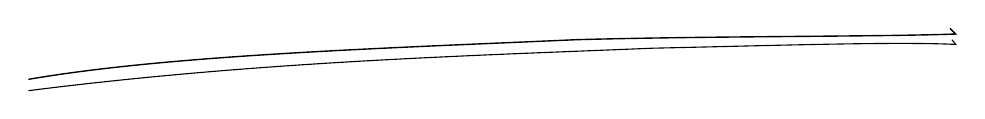
\begin{tikzpicture}[x=.012cm,y=.012cm]
\draw[line width=.5pt] (0,0) .. controls (151,26) and (379,33) .. (580,42)
  .. controls (725,46) and (896,45) .. (982,48) -- (976,54);
\draw[line width=.4pt] (0,-12) .. controls (244,19) and (468,25) .. (661,33)
  .. controls (797,36) and (918,40) .. (982,37) -- (978,42);
\end{tikzpicture}}

% Isolated faint bent stroke at the left of the pencil reference; function unknown.
\reversemarginpar
\margin{\begin{tikzpicture}[x=1mm,y=1mm]\draw[line width=.3pt] (0,0)--(.1,.7)--(.9,.5);\end{tikzpicture}}
\normalmarginpar
\handwritten{SGA 4 $\overline{\text{\uline{IX}}}$\quad p. 42\qquad note \uline{pour} la p. 8}

\figure{\begin{tikzpicture}[x=.012cm,y=.012cm]
\draw[line width=.4pt] (0,0) .. controls (270,25) and (489,51) .. (697,57)
  .. controls (814,61) and (920,63) .. (1000,67);
\end{tikzpicture}}

\handwritten{$\overline{\text{\uline{VII}}}$\quad 2.1 c)\qquad (p. 9)\quad \uline{corriger}}
% archive sheet number: 23
